\documentclass{beamer}

\mode<presentation>
{
  \usetheme{default}      % or try Darmstadt, Madrid, Warsaw, ...
  \usecolortheme{default} % or try albatross, beaver, crane, ...
  \usefonttheme{default}  % or try serif, structurebold, ...
  \setbeamertemplate{navigation symbols}{}
  \setbeamertemplate{caption}[numbered]
} 

\usepackage[english]{babel}
\usepackage[utf8]{inputenc}
\usepackage[T1]{fontenc}
\usepackage{modiagram}
\usepackage{amsmath}
\usepackage{graphicx}

\title[Your Short Title]{IChO 2020}
\author{L.F. Pa\v{s}teka}


\begin{document}

\begin{frame}
  \titlepage
\end{frame}


\begin{frame}{Schr\"{o}dingerova rovnica - voľná častica}
\begin{align*}
\hat{H} \Psi(x) = E \Psi(x) \\
-\frac{\hbar^2}{2m} \frac{d^2\Psi}{dx^2} = E \Psi \\
-\frac{\hbar^2}{2m} \nabla^2\Psi = E \Psi \\
\nabla^2\Psi = -\frac{2mE}{\hbar^2} \Psi \\
\Psi = A \cos(kx) + B \sin(kx)\\
k=\frac{\sqrt{2mE}}{\hbar}
\end{align*}
\end{frame}


\begin{frame}{Schr\"{o}dingerova rovnica - potenciálová jama}
\begin{align*}
\hat{H} \Psi = E \Psi \\
-\frac{\hbar^2}{2m} \nabla^2\Psi +\textcolor{red}{V\Psi} = E \Psi \\
V(x)=0 \quad pre \quad 0<x<L, \quad inak \quad V(x)=\infty
\end{align*}

V jame: $\Psi = A \cos(kx) + B \sin(kx)$

Mimo jamy: $\Psi = 0$
\end{frame}


\begin{frame}{Schr\"{o}dingerova rovnica - okrajové podmienky}
\begin{align*}
\Psi(0)=\Psi(L)=0 \\
\rightarrow A = 0 \\
\rightarrow k L=n\pi \\
k=\frac{n\pi}{L}=\frac{\sqrt{2mE}}{\hbar}\\
E=\frac{\hbar^2n^2\pi^2}{2mL^2}=\boxed{\frac{h^2n^2}{8mL}}
\end{align*}
\end{frame}


\begin{frame}{Úlohy - potenciálová jama}
\textbf{18.1}
\begin{align*}
E_{kv}=\frac{h^2}{8mL^2}=\frac{6.626^2}{8 \times 9.1094 \times 8^2 \times 1.4^2} 10^{-34-34+10+10+31}\\
E_{kv}=4.80 \times 10^{-20} J \\
E_n=E_{kv} n^2
\end{align*}

\textbf{18.2}
\begin{align*}
E_{tot} = 2(1+4+9+16) E_{kv} = 2.88 \times 10^{-18} J
\end{align*} 

\textbf{18.3}
\begin{align*}
E_{gap} = (25-16) E_{kv} = 4.32 \times 10^{-19} J \\
c=\lambda\nu \quad E=h\nu \quad \rightarrow \quad \lambda=\frac{h c}{E_{gap}} = 460 \: nm
\end{align*} 
\end{frame}


\begin{frame}{Úlohy - potenciálová jama}
\textbf{18.4}
\begin{align*}
A_{lattice} = (11 \text{\AA})^2 = 1.21 \times 10^{-18} \: m^2\\
A_{hex} = \frac{3\sqrt{3}}{2}L^2 = 5.09 \times 10^{-20} \: m^2\\
N_{hex} = \frac{A_{lattice}}{A_{hex}} \approx 24 \quad \rightarrow \quad 48 e^- \quad \rightarrow \quad 24 \: MO
\end{align*} 

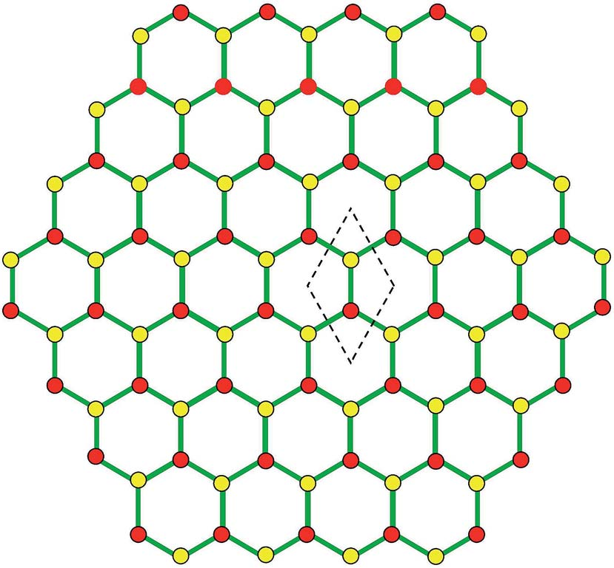
\includegraphics[width=3cm]{hex_lattice.png} 2 uhlíky na 1 šesťuholník
\end{frame}

\begin{frame}{Úlohy - potenciálová jama}
\textbf{18.5-7}

pozri excelovský hárok!

\begin{align*}
E=E_{kv}(n_1^2+n_2^2) \quad kde \quad E_{kv}=\frac{h^2}{8mL_1^2}=4.98 \times 10^{-20} J \\
E_{HOMO}=E_{kv}(1^2+6^2)=37 E_{kv} = 1.84 \times 10^{-18} J \\
E_{LUMO}=E_{kv}(2^2+6^2)=40 E_{kv} = 1.99 \times 10^{-18} J \\
E_{gap}=(40-37)E_{kv} = 1.5 \times 10^{-19} J
\end{align*} 
\end{frame}


\begin{frame}{Úlohy - potenciálová jama}
\textbf{18.8-9}

podobne
\begin{align*}
E_{n_1n_2n_3}=E_{kv}(n_1^2+n_2^2+n_3^3) \quad kde \quad E_{kv}=\frac{h^2}{8mL^2} \\
E_{111}=3E_{kv} \quad 1\times deg.\\
E_{112}=E_{121}=E_{211}=6E_{kv} \quad 3\times deg.\\
E_{122}=E_{212}=E_{221}=9E_{kv} \quad 3\times deg.
\end{align*} 
atď.
\end{frame}


\begin{frame}{Úlohy - harmonický oscilátor}
\textbf{19.1-3}
\begin{align*}
\mu = \frac{12 \times 16 }{12+16} = 6.86\: amu = 1.14 \times 10^{-26} \: kg\\
\nu = \frac{1}{2\pi}\sqrt{\frac{k}{\mu}} = 65 \: THz \\
\tilde{\nu}=\frac{1}{\lambda}=\frac{\nu}{c}=2170 \: cm^{-1} \\
E_{ZPV}=\frac{1}{2}h\nu=2.16\times 10^{-20} J = 3.1 kcal/mol
\end{align*}
\end{frame}


\begin{frame}{Úlohy - harmonický oscilátor}
\textbf{19.4}
\begin{align*}
\frac{\nu_2}{\nu_1} = \frac{\frac{1}{2\pi}\sqrt{\frac{k}{\mu_2}}}{\frac{1}{2\pi}\sqrt{\frac{k}{\mu_1}}} = \sqrt{\frac{\mu_1}{\mu_2}} \quad \rightarrow \quad \nu_2=\sqrt{\frac{\mu_1}{\mu_2}} \nu_1\\
\frac{\mu_1}{\mu_2}=\frac{\frac{12\times16}{12+16}}{\frac{13\times16}{13+16}} = \frac{12\times 29}{13\times 28} = 0.956 \quad \rightarrow \quad \sqrt{\frac{\mu_1}{\mu_2}} = 0.978\\
\tilde{\nu}_2=0.978\:\tilde{\nu}_1=0.978\times2170=2122 \: cm^{-1}\\
\end{align*}

\textbf{19.5}
\begin{align*}
\frac{\mu_1}{\mu_2}= \frac{16\times 29}{17\times 28} = 0.975 \quad \rightarrow \quad \sqrt{\frac{\mu_1}{\mu_2}} = 0.987\\
\tilde{\nu}_2=0.987\:\tilde{\nu}_1=0.987\times2170=2142 \: cm^{-1}\\
\end{align*}
\end{frame}


\begin{frame}{Úlohy - harmonický oscilátor}
\textbf{19.6}
\begin{align*}
\tilde{\nu}_{ZPV}=\frac{1}{2}(1649+3832+3942)=4712\: cm^{-1}\\
E_{ZPV}=hc_{ZPV}=9.36\times 10^{-20} \:J
\end{align*}

\textbf{19.7}

\begin{tabular}{ccccccccccc}
&$\nu_1$&$\nu_2$&$\nu_3$\\
$\times$&0&0&0&=&0   &+&$\tilde{\nu}_{ZPV}$&=&4712 cm$^{-1}$ \\
$\times$&1&0&0&=&1649&+&$\tilde{\nu}_{ZPV}$&=&6361 cm$^{-1}$  \\
$\times$&2&0&0&=&3298&+&$\tilde{\nu}_{ZPV}$&=&8010 cm$^{-1}$  \\
$\times$&0&1&0&=&3832&+&$\tilde{\nu}_{ZPV}$&=&8544 cm$^{-1}$  \\
$\times$&0&0&1&=&3943&+&$\tilde{\nu}_{ZPV}$&=&8655 cm$^{-1}$
\end{tabular}
\end{frame}

\begin{frame}{Úlohy - tuhý rotor}
\textbf{19.8}

prepokladáme, že $R$ nezávisí od izotopov
\begin{align*}
\Delta E=E_1-E_0=\frac{h^2}{8\pi^2I}\left[1(1+1)-0(0+1)\right]=\frac{h^2}{4\pi^2I}\\
\Delta E=h\nu=\frac{h^2}{4\pi^2\mu R^2} \quad \rightarrow \quad R=\sqrt{\frac{h}{4\pi^2\mu\nu}}=\frac{1}{2\pi}\sqrt{\frac{h}{\mu\nu}}=1.13\text{\AA}
\end{align*}
($\mu$ už máme z úlohy 19.1)
\\
\textbf{19.9}
\begin{align*}
\nu_{l+1}-\nu_{l}=\frac{h}{8\pi^2I}\left[(l+1)(l+2)-l(l+1)\right]=\frac{h}{4\pi^2I}(l+1)\\
\rightarrow \nu_{2-1}=2\times115=230\: GHz\\
\rightarrow \nu_{3-2}=3\times115=345\: GHz\\
\end{align*}
\end{frame}


\begin{frame}{Úlohy - tuhý rotor}
\textbf{19.10}
\begin{align*}
\frac{\nu_2}{\nu_1}=\frac{\frac{h}{8\pi^2\mu_2R^2}}{\frac{h}{8\pi^2\mu_1R^2}}=\frac{\mu_1}{\mu_2} \quad \rightarrow \quad \nu_2=\frac{\mu_1}{\mu_2} \nu_1\\
\frac{\mu_1}{\mu_2}=0.975 \quad (\text{poznáme z úlohy 19.5})\\
\nu_2=0.975\times115=112\: GHz
\end{align*}
\end{frame}
 
 \end{document}
